\documentclass[8pt]{beamer}

\usepackage[T1]{fontenc}
\usepackage [utf8]{inputenc}
\usepackage [polish]{babel}
\usepackage{hyperref}

\usepackage{graphicx}

\usetheme{Berlin}

\title{Konsolowe technologie i ich historia}
\author{Adrian Dopart}
\date{\today}

\begin{document}

\begin{frame}
    \titlepage
\end{frame}

\begin{frame}
\frametitle{Czym jest konsola do gier?}
\textbf{Konsola do gier} - specjalne urządzenie przeznaczone do uruchamiania gier wideo na ekranie telewizora lub monitora. Jest to sprzęt zaprojektowany wyłącznie z myślą o grach, w odróżnieniu od komputerów osobistych (PC), które pełnią wiele różnych funkcji.

\textbf{Cechy charakterystyczne konsoli do gier:}

\begin{itemize}
\item \textbf{Dedykowany system operacyjny} zoptymalizowany pod kątem gier.
\item \textbf{Prosta obsługa} – konsola jest gotowa do działania po podłączeniu do telewizora.
\item \textbf{Kontrolery} dostosowane do różnych gatunków gier (gamepady, kontrolery ruchowe).
\item \textbf{Ekskluzywne tytuły} – gry dostępne tylko na konkretną platformę (np. Uncharted dla PlayStation, Halo dla Xbox).

\end{itemize}

\end{frame}

\begin{frame}
\frametitle{Początki konsol do gier}
Pierwsze konsole pojawiły się na początku lat 70. XX wieku. Oto kluczowe momenty z początków historii konsol:
\textbf{Magnavox Odyssey (1972)}

\begin{itemize}
\item \textbf {Pierwsza komercyjna konsola} na świecie.
\item Została zaprojektowana przez \textbf{Ralpha Baera}.
\item Gry były bardzo proste, a grafika ograniczała się do prostych figur geometrycznych wyświetlanych na ekranie telewizora.

\end{itemize}

\textbf{Atari 2600 (1977)}
\begin{itemize}
\item Jedna z najważniejszych konsol drugiej generacji.
\item Wprowadziła wymienne kartridże, co pozwalało na zakup nowych gier bez zmiany sprzętu.
\item \textbf {Popularne tytuły:} \textit {Space Invaders, Pac-Man, Adventure.}

\end{itemize}

\end{frame}

\begin{frame}
\frametitle{Początki konsol do gier}
Po premierze \textbf {Magnavox Odyssey} w 1972 roku i \textbf {Atari 2600} w 1977 roku pojawiło się wiele kolejnych konsol, które wpłynęły na rozwój rynku gier wideo.

\textbf {Fairchild Channel F (1976) }
\begin{itemize}
\item \textbf {Pierwsza konsola z wymiennymi kartridżami.}
\item Używała mikroprocesora, co było rewolucyjnym krokiem w stosunku do wcześniejszych konsol.
\item Gry były proste, ale różnorodne – od gier sportowych po logiczne.

\end{itemize}

\textbf {Atari 5200 (1982)}
\begin{itemize}
\item Następca Atari 2600 z lepszą grafiką i dźwiękiem.
\item Niestety nie odniósł sukcesu z powodu skomplikowanych kontrolerów i problemów z kompatybilnością.

\end{itemize}

\end{frame}

\begin{frame}
\frametitle{Początkowe konsole}
    \begin{figure}[ht]
        \begin{minipage}[b]{0.45\linewidth}
            \centering
            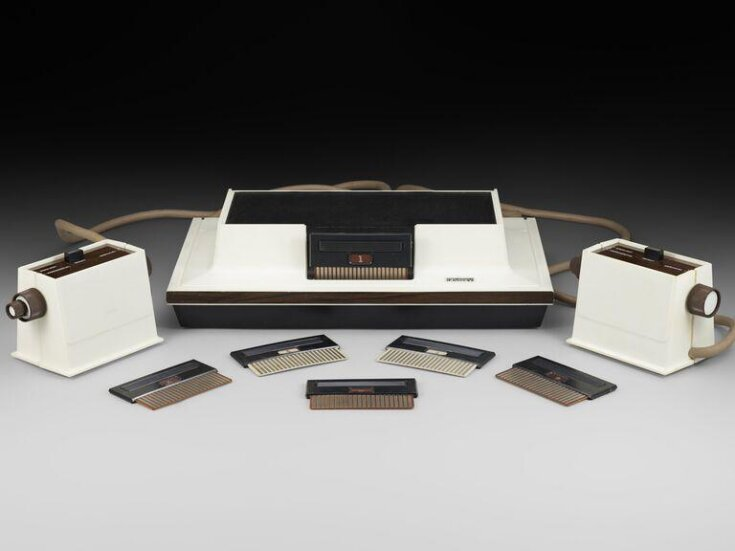
\includegraphics[width=\textwidth]{magnafox.jpg}
	    \caption{Magnafox Odyssey}
            \label{fig:a}
        \end{minipage}
        \hspace{0.5cm}
        \begin{minipage}[b]{0.45\linewidth}
            \centering
            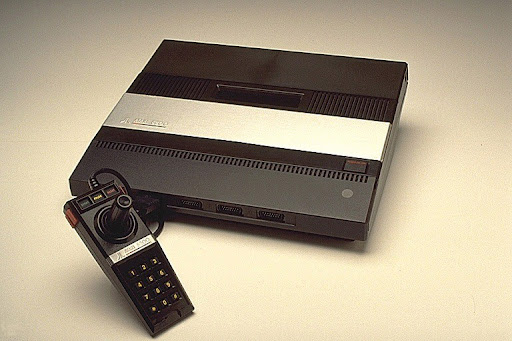
\includegraphics[width=\textwidth]{atari5200.jpg}
            \caption{Atari 5200}
            \label{fig:b}
        \end{minipage}
    \end{figure}
\end{frame}


\begin{frame}
\frametitle{Era 8-bitowa i kryzys gier wideo}
Na początku lat 80. rynek gier przeżywał boom, ale doszło też do tzw. \textbf {kryzysu gier wideo w 1983 roku.} Przyczynami były:
\begin{itemize}
\item \textbf {Niska jakość gier} – wiele gier było wydawanych w pośpiechu, bez odpowiedniej kontroli jakości.
\item \textbf {Przesycenie rynku} – zbyt wiele firm próbowało tworzyć konsole i gry, co doprowadziło do chaosu i spadku zainteresowania graczy.
\item Kryzys zakończył się wraz z premierą \textbf {Nintendo Entertainment System (NES)} w 1985 roku, który przywrócił wiarę w jakość gier i zapoczątkował nową erę konsol 8-bitowych.
\end{itemize}
\end{frame}


\begin{frame}
\frametitle{Dalszy rozwój konsol - Genesis}
\begin{columns}

    \begin{column}{0.6\textwidth}
        Po przełomowych konsolach lat 80., takich jak \textbf{NES i Sega Master System}, technologia zaczęła rozwijać się w szybkim tempie, prowadząc do wprowadzenia nowych funkcji, lepszej grafiki oraz innowacji w rozgrywce.
        
        \vspace{0.5em}
        \textbf{Sega Mega Drive / Genesis (1988)} – była konsolą 16-bitową.
        \begin{itemize}
            \item Konkurent dla NES-a i późniejszego SNES-a.
            \item Popularne tytuły: \textit{Sonic the Hedgehog, Streets of Rage, Golden Axe}.
        \end{itemize}
    \end{column}

    \begin{column}{0.35\textwidth}
        \centering
        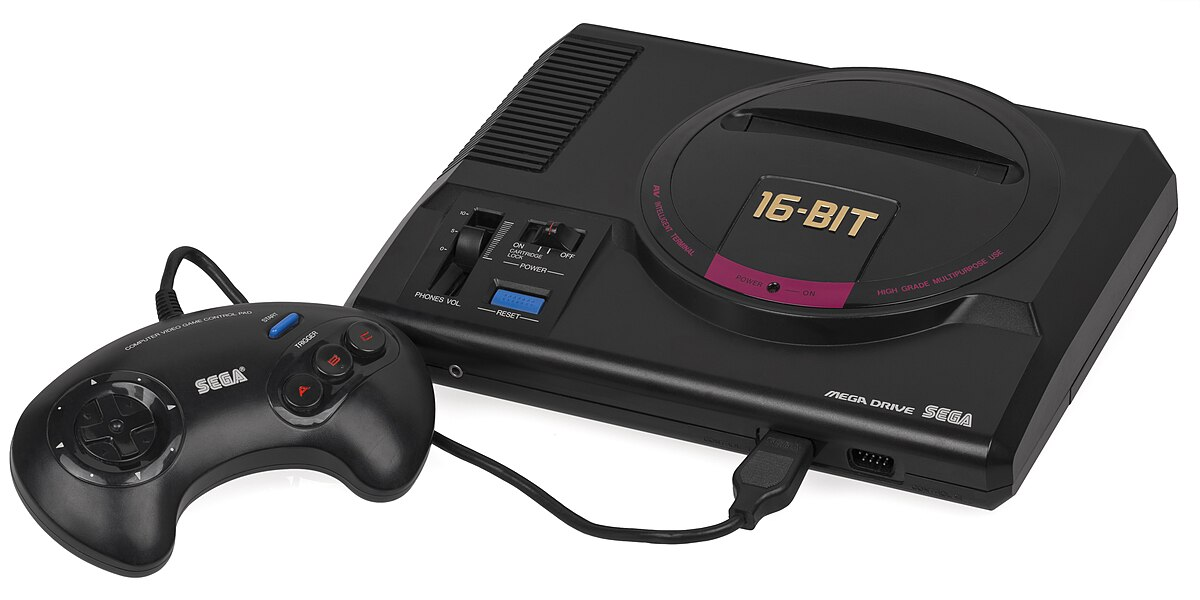
\includegraphics[width=\textwidth]{sega.jpg} 
        {\small Sega Genesis} 
    \end{column}
\end{columns}
\end{frame}

\begin{frame}
\frametitle{Sony PlayStation}
\begin{columns}

\begin{column}{0.6\textwidth}
\textbf {Sony PlayStation (PS1)}- wydana 3 grudnia 1994 roku w Japonii (a w 1995 roku w Ameryce Północnej i Europie), była pierwszą konsolą od \textbf {Sony Computer Entertainment.} Stała się jedną z najbardziej przełomowych konsol w historii gier wideo i przyczyniła się do ogromnych zmian w przemyśle gier.

\vspace{0.5em}

Sony postanowiło stworzyć własną konsolę do gier, która wykorzystywałaby technologię CD-ROM, dzięki czemu rynek, wprowadzając gry na płytach CD, co pozwoliło na większą pojemność i lepsze efekty dźwiękowe oraz graficzne.
\end{column}

\begin{column}{0.35\textwidth}
        \centering
        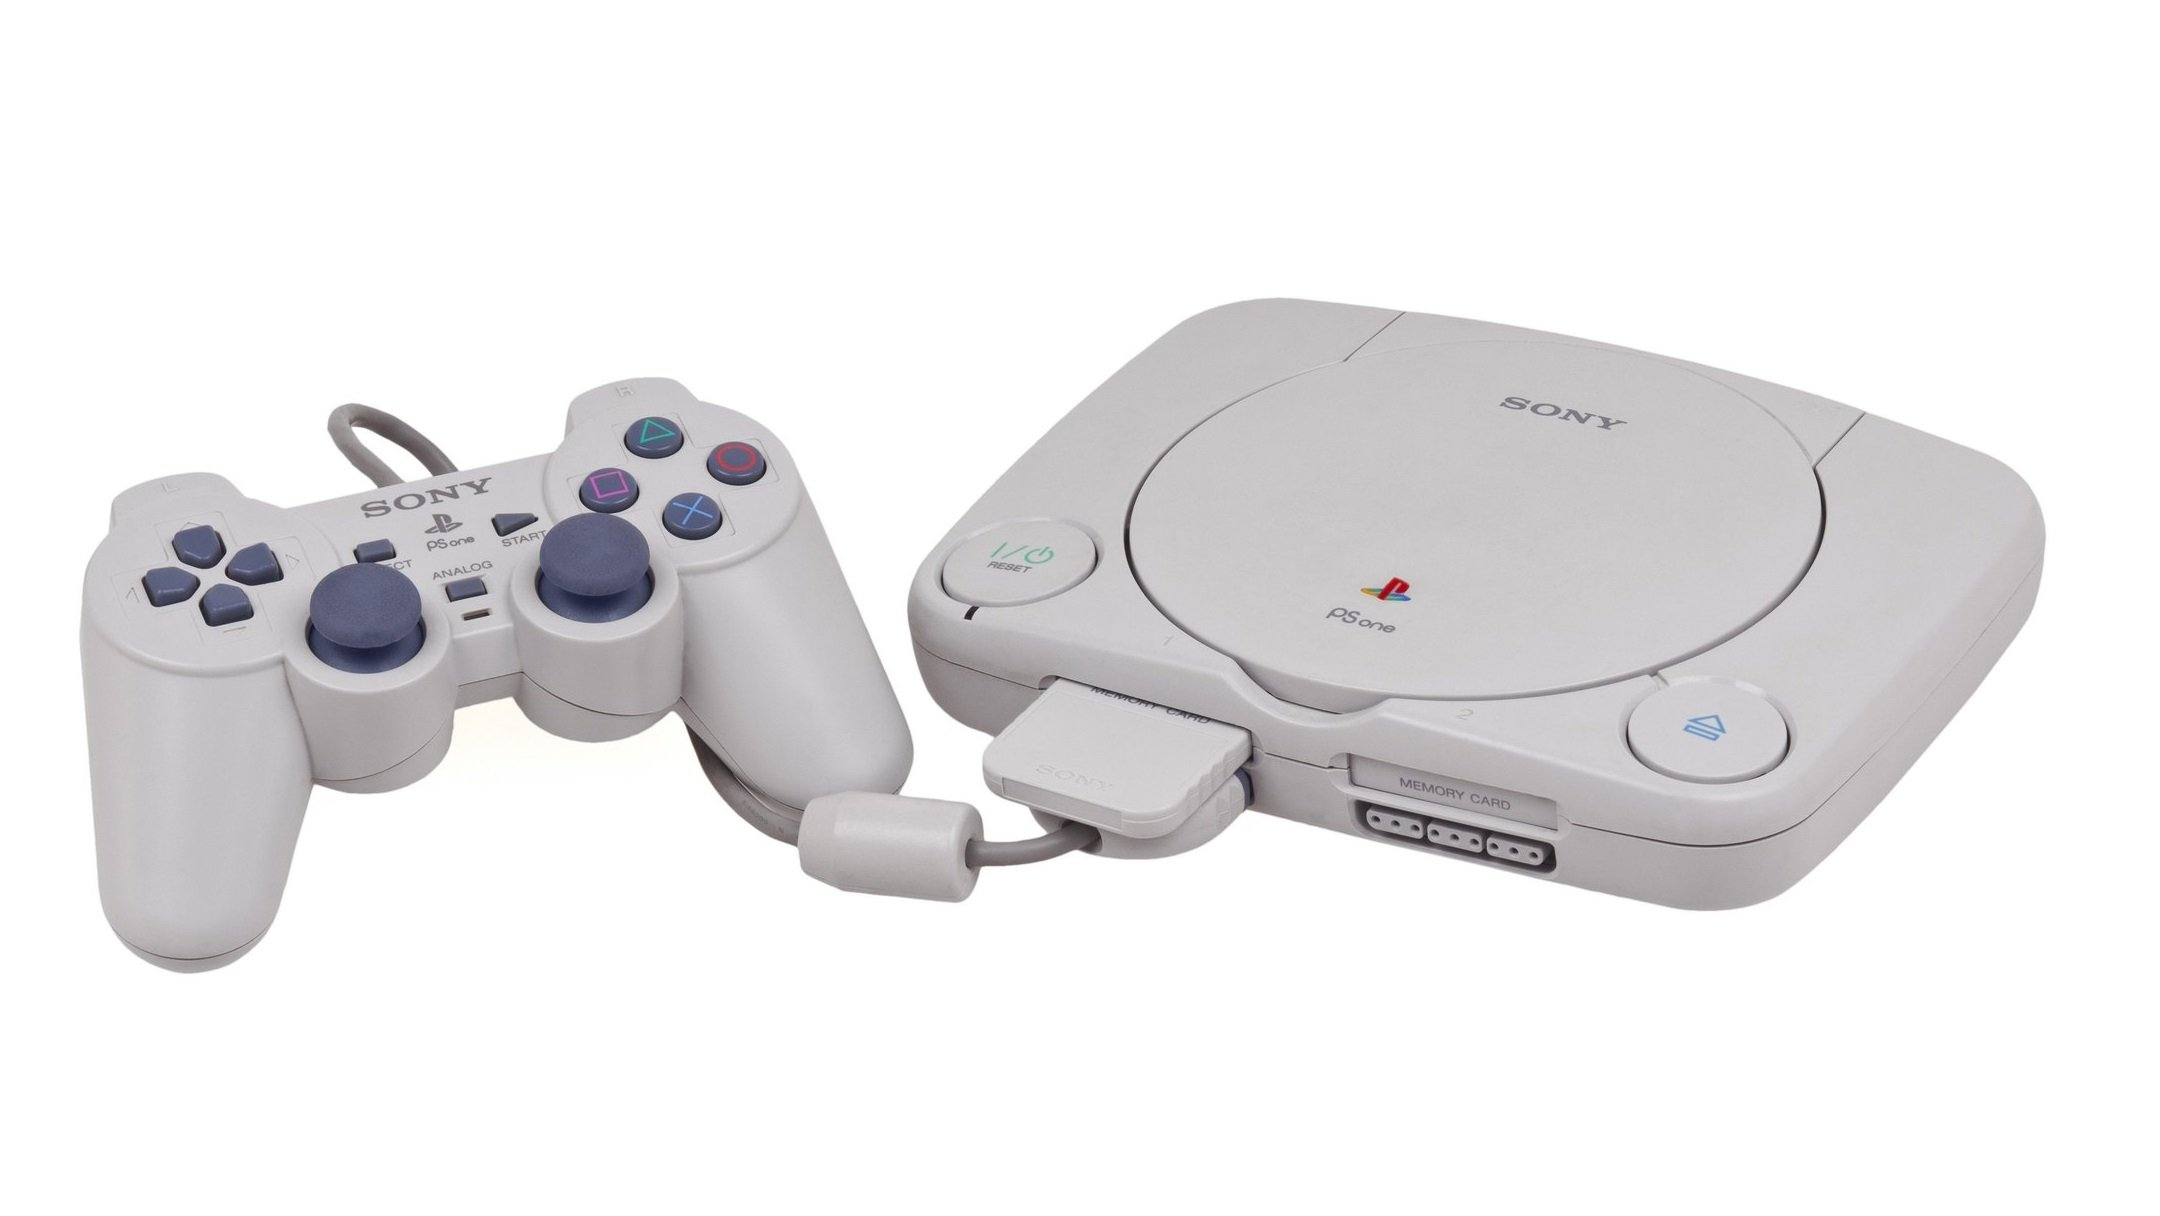
\includegraphics[width=\textwidth]{ps1.jpg} 
        {\small PlayStation 1} 
    \end{column}
\end{columns}

\end{frame}

\begin{frame}
\frametitle{Nintendo 64 – odpowiedź na PS1}
\begin{columns}

\begin{column}{0.6\textwidth}
\textbf {Nintendo 64}, często nazywane N64, to konsola wydana przez Nintendo w 1996 roku (w Japonii i Ameryce Północnej) oraz w 1997 roku w Europie.
 
\vspace{0.5em}

Była to pierwsza konsola Nintendo, która obsługiwała gry w pełnym 3D. Oferowała zaawansowaną grafikę 3D z teksturami i efektami specjalnymi, takimi jak antyaliasing (wygładzanie krawędzi).
\vspace{0.5em}

Oferowała zaawansowaną grafikę 3D z teksturami i efektami specjalnymi, takimi jak antyaliasing (wygładzanie krawędzi).

\end{column}

\begin{column}{0.35\textwidth}
        \centering
        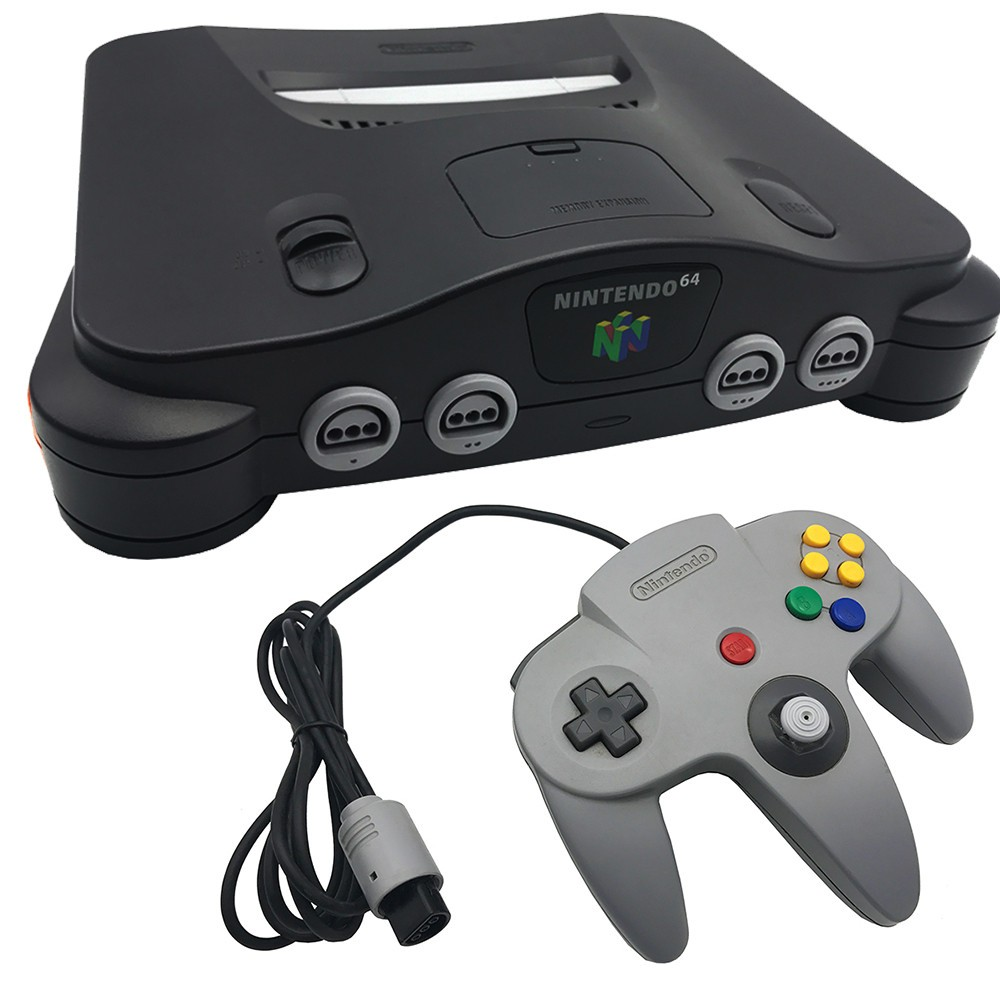
\includegraphics[width=\textwidth]{nintendo64.jpg} 
        {\small Nintendo 64} 
    \end{column}
\end{columns}
\end{frame}


\begin{frame}
\frametitle{PlayStation 2}
\begin{columns}

\begin{column}{0.6\textwidth}
\textbf {PlayStation 2}- wydana przez Sony Computer Entertainment. Została wydana 4 marca 2000 roku w Japonii, a później tego samego roku w Ameryce Północnej i Europie. PS2 była jedną z najważniejszych konsol w historii gier wideo i do dziś pozostaje najlepiej sprzedającą się konsolą wszech czasów z liczbą ponad 155 milionów sprzedanych egzemplarzy.

\vspace{0.5em}

PS2 była nie tylko konsolą do gier, ale także \textbf {odtwarzaczem DVD}, co sprawiło, że była atrakcyjna dla szerszego grona odbiorców. W czasach gdy odtwarzacze DVD były drogie, PS2 oferowała tą funkcję w przystępnej cenie.
\vspace{0.5em} 
Wersje konsoli PS2:
\begin{itemize}
\item PlayStation 2 (Fat)
\item PlayStation 2 Slim (2004)
\end{itemize}
\end{column}

\begin{column}{0.35\textwidth}
        \centering
        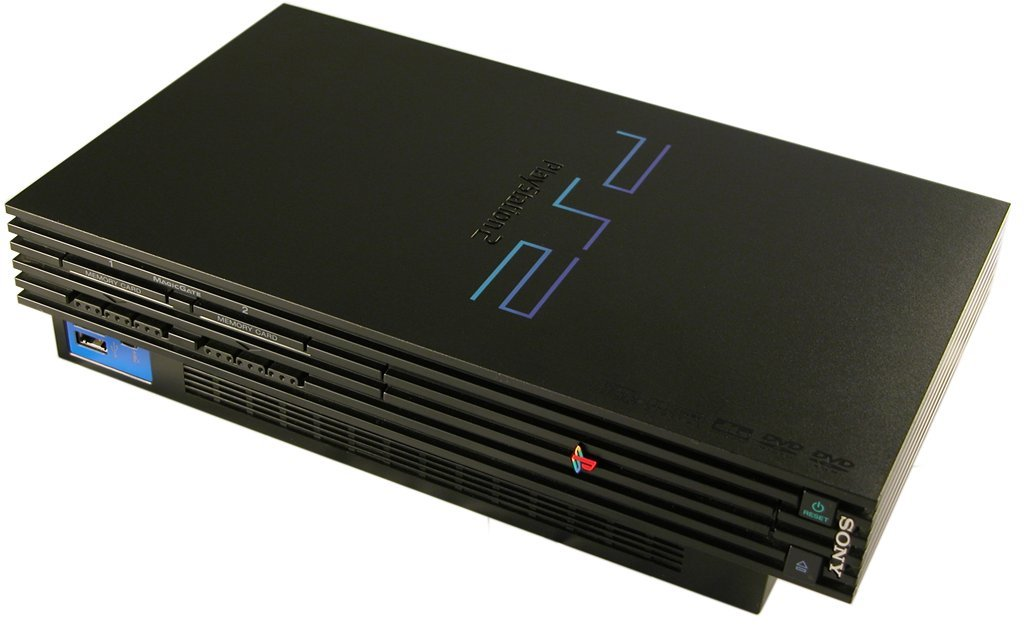
\includegraphics[width=\textwidth]{PS2.jpg} 
        {\small PlayStation 2} 
    \end{column}
\end{columns}

\end{frame}

\begin{frame}{Xbox (2001}
\frametitle{Xbox (2001)}
\begin{columns}

\begin{column}{0.6\textwidth}
\textbf {Xbox} to pierwsza konsola stacjonarna stworzona przez Microsoft, wydana 15 listopada 2001 roku w Ameryce Północnej, a później w 2002 roku w Japonii, Europie i Australii. 
\vspace{0.5em}
Xbox był odpowiedzią Microsoftu na dominację \textbf {Sony PlayStation 2.} Konsola wyróżniała się zaawansowaną specyfikacją techniczną, nowatorskimi funkcjami online oraz wprowadzeniem kultowej serii \textbf {„Halo”.}
\vspace{0.5em}
Xbox wprowadził nowatorską usługę online – \textbf {Xbox Live.}
Umożliwiała grę wieloosobową przez internet, komunikację głosową oraz pobieranie dodatkowej zawartości. Wprowadziła jednolity system kont gracza oraz listę znajomych.
\end{column}

\begin{column}{0.35\textwidth}
        \centering
        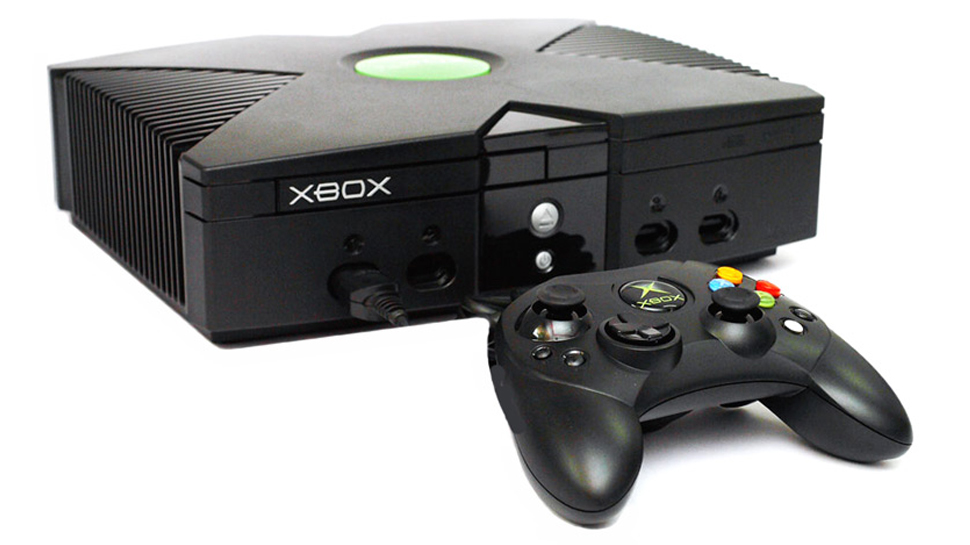
\includegraphics[width=\textwidth]{xbox.jpg} 
        {\small Xbox (2001)} 
    \end{column}
\end{columns}

\end{frame}

\begin{frame}
\frametitle{Nintendo Wii}
\begin{columns}

\begin{column}{0.6\textwidth}
\textbf {Nintendo Wii} - wydana przez Nintendo 19 listopada 2006 roku w Ameryce Północnej, a następnie w Japonii, Europie i Australii. 
Wii była przełomem w świecie gier dzięki innowacyjnemu systemowi sterowania ruchowego, który przyciągnął nie tylko graczy, ale również osoby wcześniej nieinteresujące się grami. Konsola stała się ogromnym sukcesem komercyjnym i sprzedała się w ponad 101 milionach egzemplarzy na całym świecie.

\vspace{0.5em}
Najważniejszym elementem Wii był kontroler \textbf{Wii Remote (Wiimote).} Dzięki czujnikom ruchu i technologii żyroskopowej można było sterować grami poprzez wykonywanie gestów i ruchów. Konsola wykorzystywała sensor bar, który śledził położenie kontrolera w przestrzeni.

\end{column}

\begin{column}{0.35\textwidth}
        \centering
        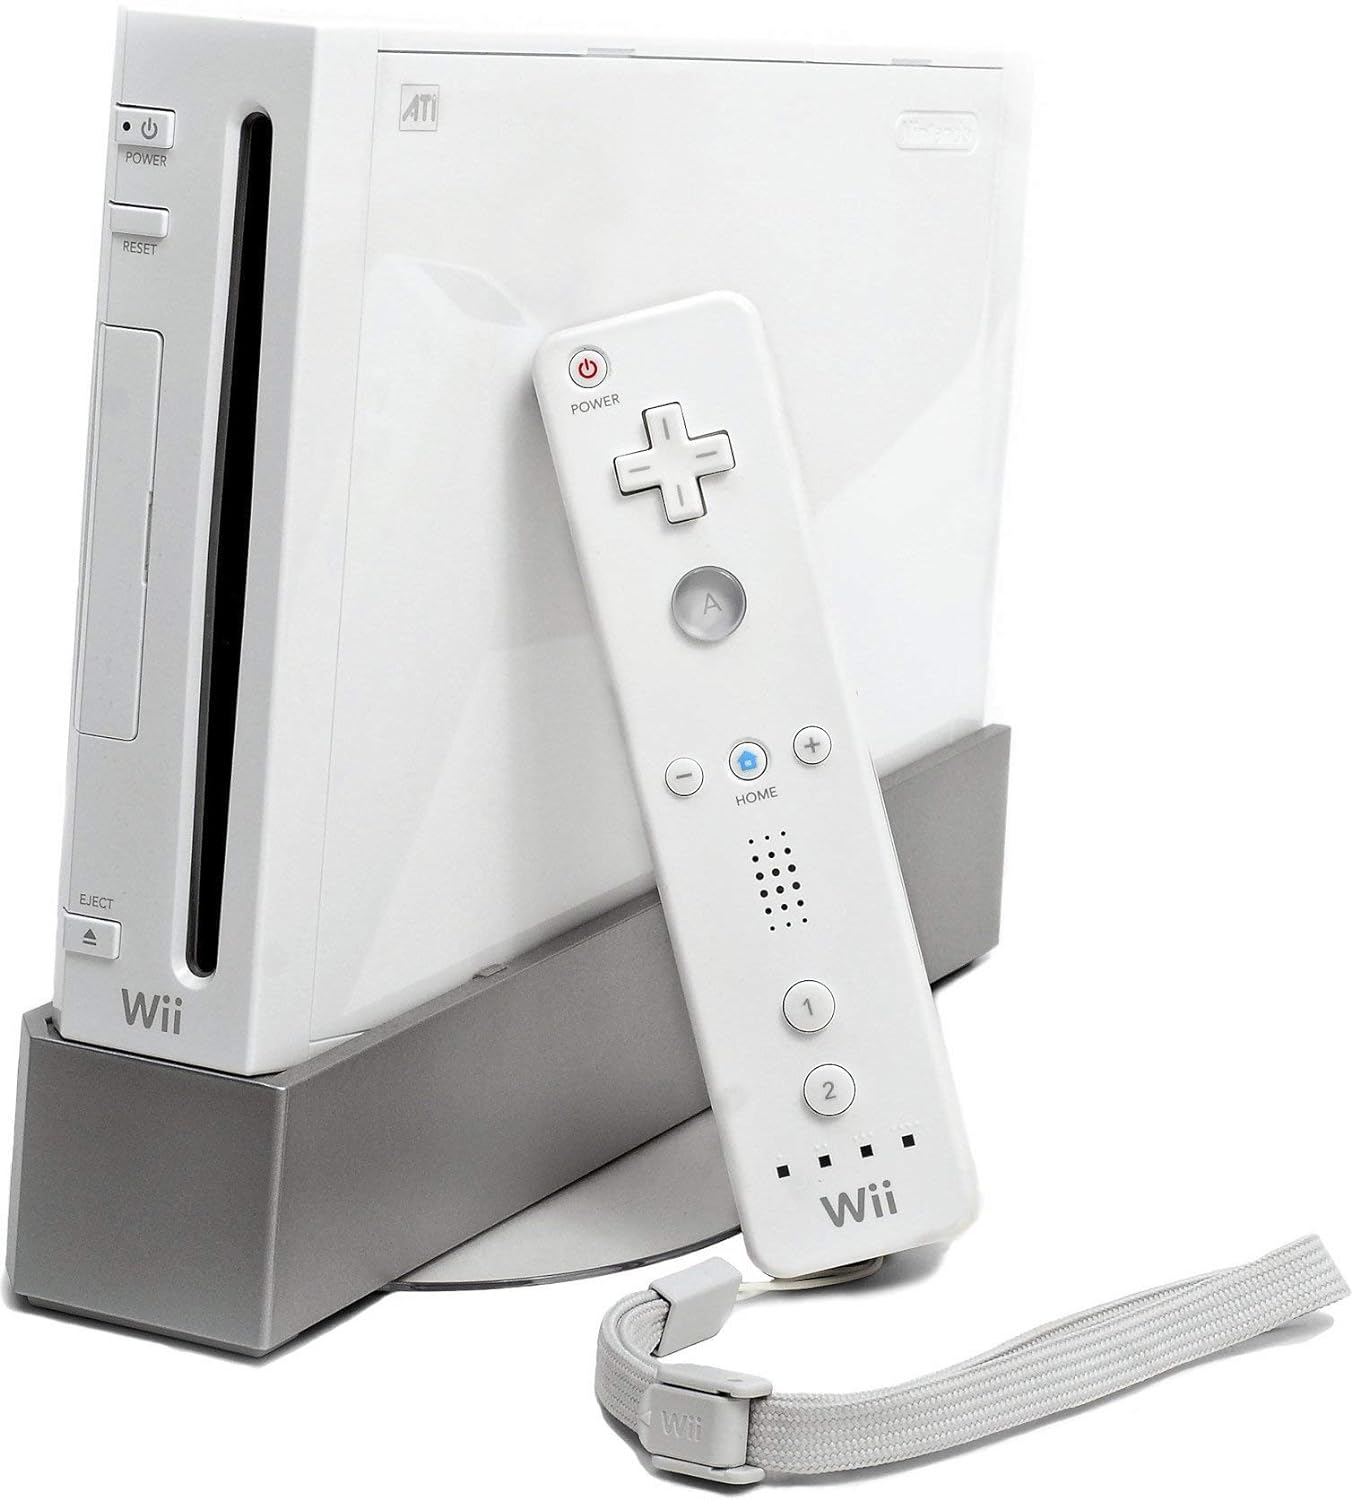
\includegraphics[width=\textwidth]{wii.jpg} 
        {\small Nintendo Wii} 
    \end{column}
\end{columns}

\end{frame}

\begin{frame}
\frametitle{PlayStation 3}
\begin{columns}

\begin{column}{0.6\textwidth}
\textbf {PlayStation 3} – konsola siódmej generacji stworzona przez Sony Computer Entertainment. Została wydana 11 listopada 2006 roku w Japonii, a następnie w Ameryce Północnej, Europie i Australii.

\vspace{0.5em}
PS3 była odpowiedzią Sony na rosnącą konkurencję ze strony Microsoft Xbox 360 i Nintendo Wii. PS3 wyróżniała się zaawansowaną specyfikacją techniczną, wbudowanym odtwarzaczem Blu-ray, oraz silnym naciskiem na gry w wysokiej jakości grafice 3D.

\vspace{0.5em}
\textbf {PS3} była pierwszą konsolą do gier, która obsługiwała \textbf {Blu-ray}– nowoczesny nośnik o dużej pojemności, który mógł pomieścić do 50 GB danych. Dzięki temu, gry na PS3 mogły oferować niespotykaną wcześniej jakość grafiki i dźwięku.

\end{column}

\begin{column}{0.35\textwidth}
        \centering
        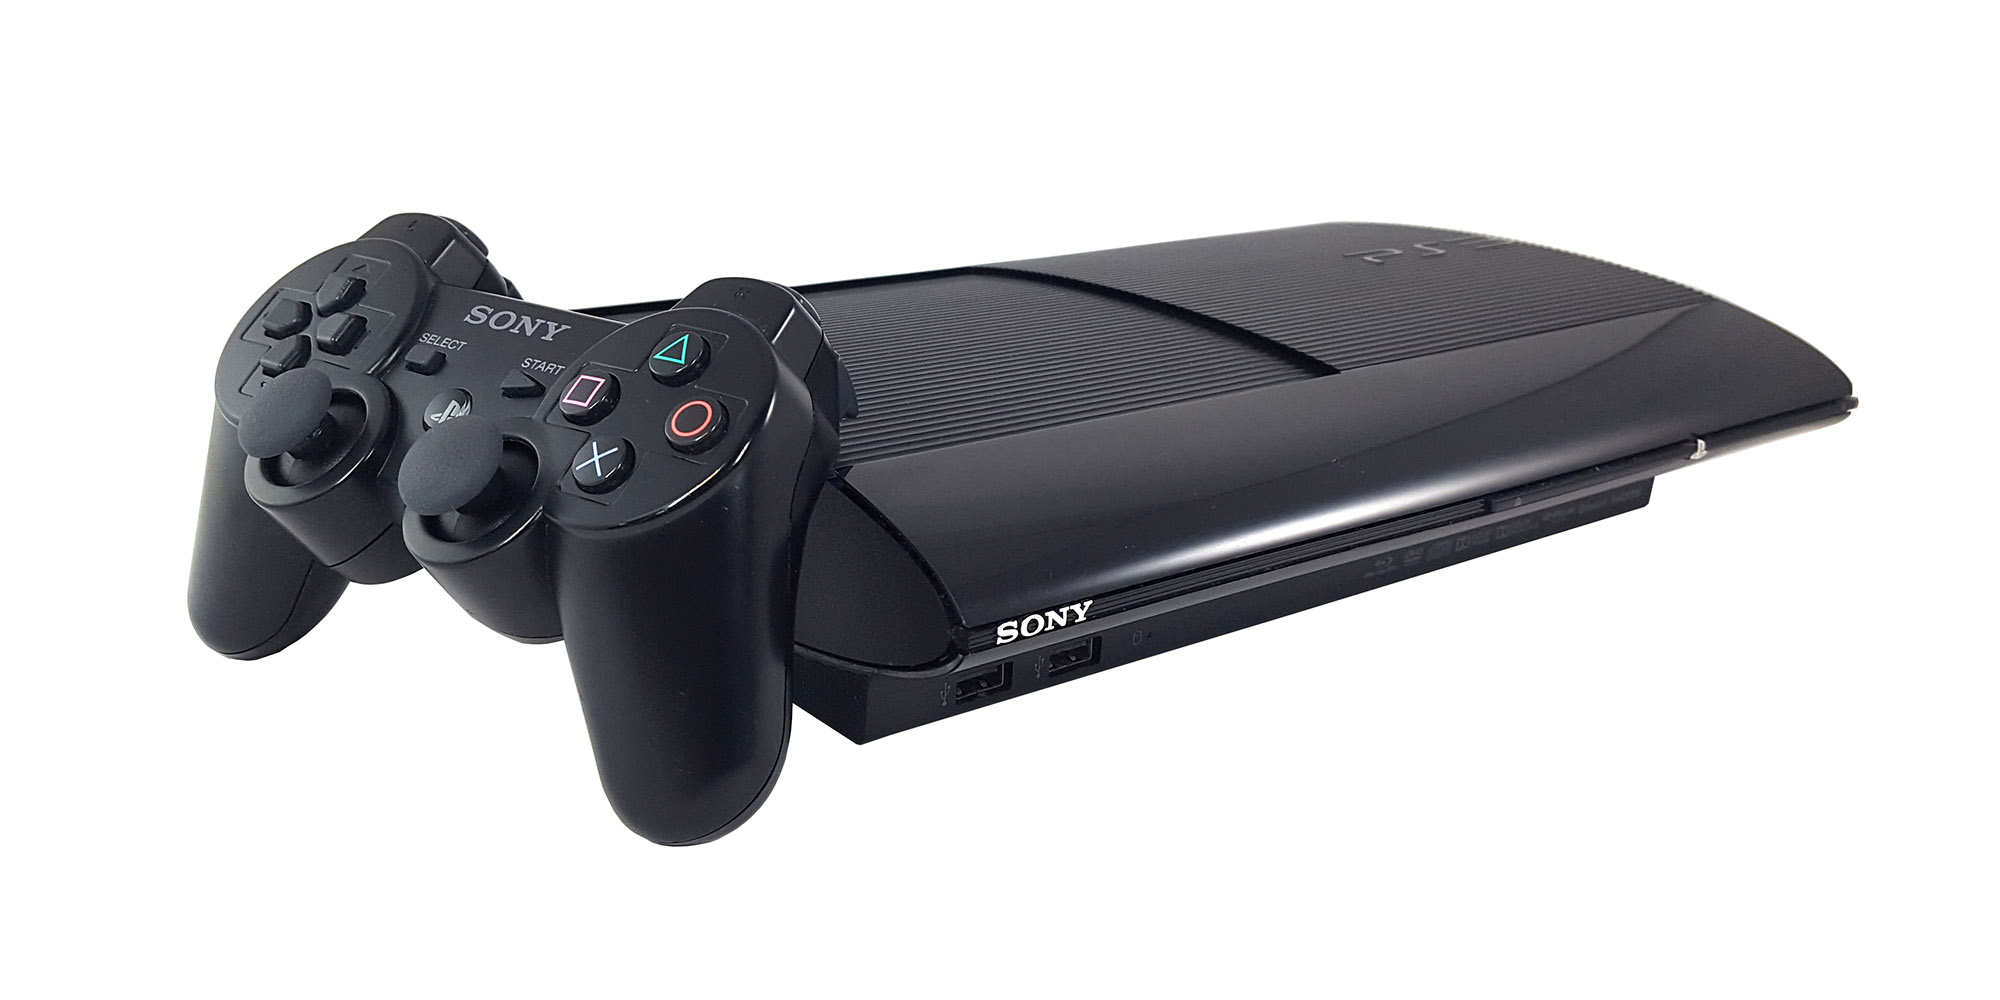
\includegraphics[width=\textwidth]{ps3.jpg} 
        {\small PlayStation 3} 
    \end{column}
\end{columns}

\end{frame}

\begin{frame}
\frametitle{PlayStation Portable (PSP)}
\begin{columns}

\begin{column}{0.6\textwidth}
\textbf {PlayStation Portable (PSP)} – przenośna konsola stworzona przez Sony Computer Entertainment i wydana 12 grudnia 2004 roku w Japonii, a potem w 2005 roku na innych rynkach. PSP była jednym z pierwszych poważniejszych prób wejścia Sony na rynek przenośnych urządzeń do gier, konkurując z takimi konsolami jak Nintendo DS.

\vspace{0.5em} 
PSP wyróżniała się zaawansowaną specyfikacją techniczną, dużym ekranem LCD i możliwością odtwarzania gier w wysokiej jakości grafice, co w tamtych czasach było rewolucyjne dla urządzeń mobilnych.

\vspace{0.5em}
PSP była pierwszą konsolą przenośną, która mogła zaoferować grafikę porównywalną z konsolami stacjonarnymi, co sprawiło, że gry na PSP wyglądały znacznie lepiej niż na innych przenośnych urządzeniach. 

\end{column}

\begin{column}{0.35\textwidth}
        \centering
        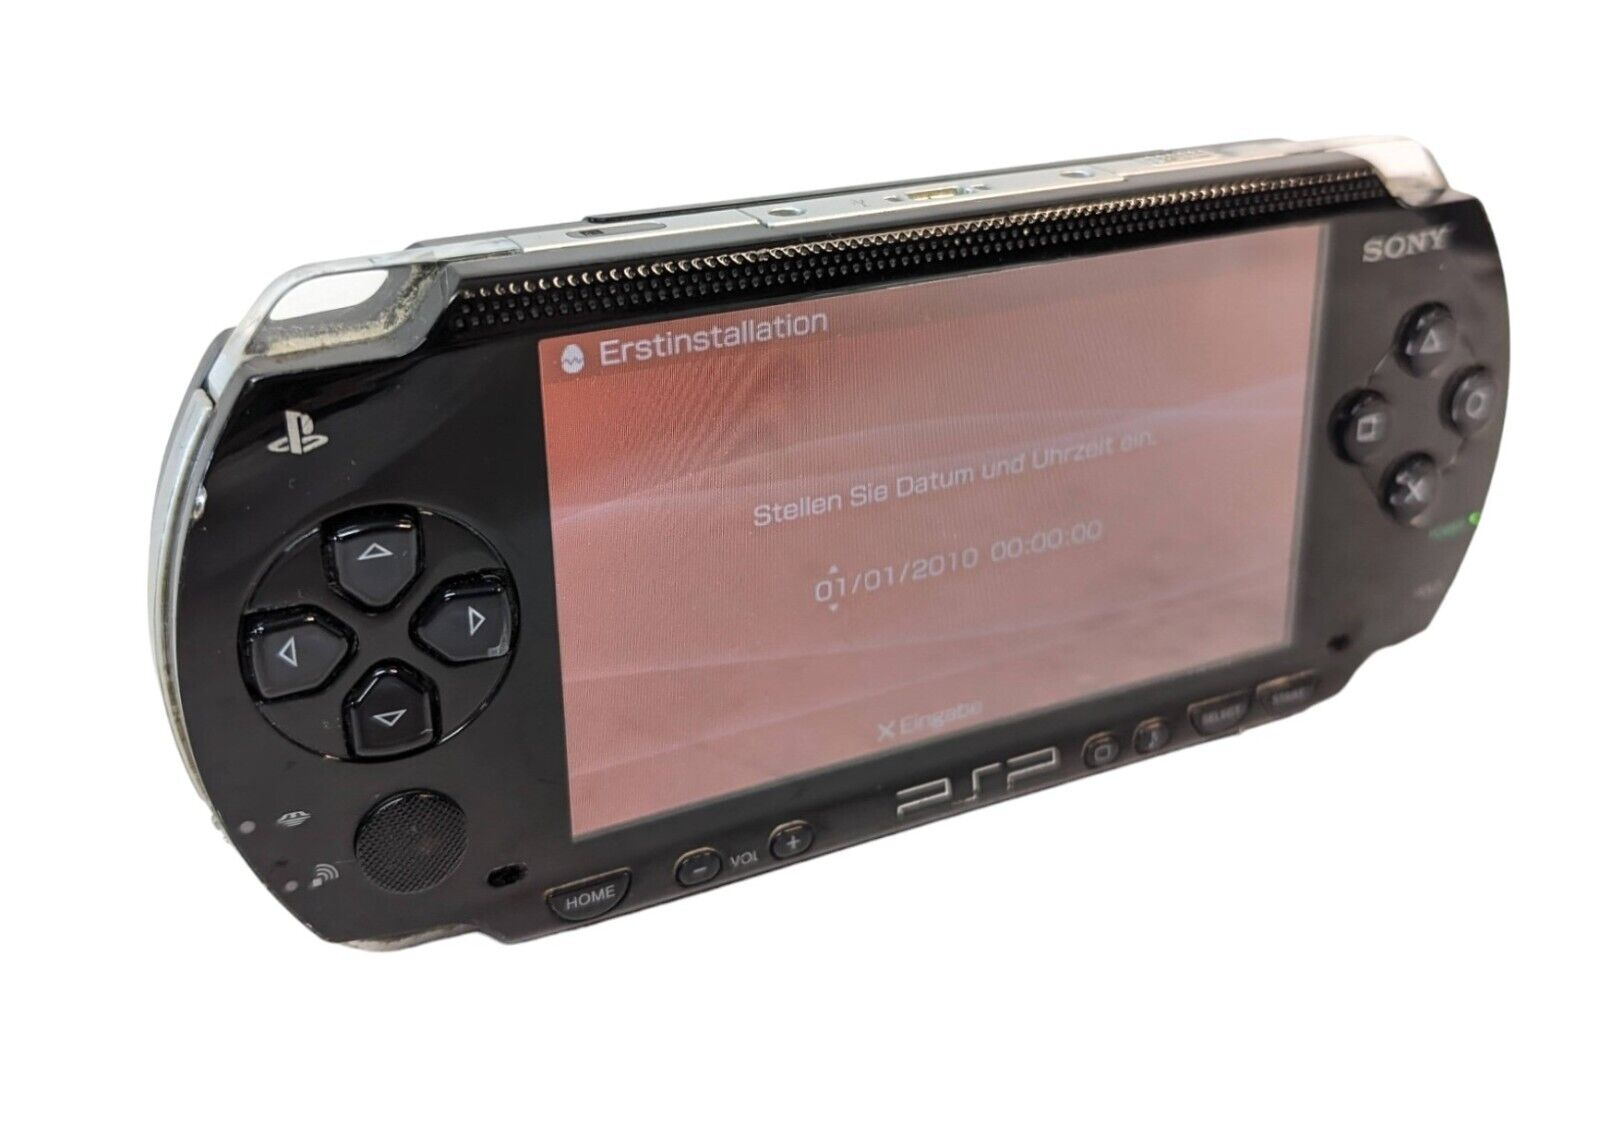
\includegraphics[width=\textwidth]{psp.jpg} 
        {\small PlayStation Portable} 
    \end{column}
\end{columns}

\end{frame}

\begin{frame}
\frametitle{Xbox 360}
\begin{columns}

\begin{column}{0.6\textwidth}
\textbf {Xbox 360} – konsola siódmej generacji wydana przez Microsoft. Została zaprezentowana 12 maja 2005 roku, a jej debiut na rynku miał miejsce 22 listopada 2005 roku w Ameryce Północnej, a potem na innych rynkach. Była to bezpośrednia konkurentka dla PlayStation 3 i Nintendo Wii. Konsola była pierwszym dużym sukcesem Microsoftu w branży gier, zdobywając ogromną bazę użytkowników i wyznaczając nowe standardy w rozrywce interaktywnej.

\vspace{0.5em} 
Xbox 360 zadebiutował z bezprzewodowym kontrolerem, który stał się jednym z najbardziej komfortowych kontrolerów w historii gier. Charakteryzował się solidnym chwytem, precyzyjnym analogiem i łatwym dostępem do przycisków.

\vspace{0.5em}
W 2010 roku, Microsoft zaprezentował \textbf {Kinect}, nowatorski system do sterowania ruchem do Xboxa 360, który nie wymagał fizycznych kontrolerów.

\end{column}

\begin{column}{0.35\textwidth}
        \centering
        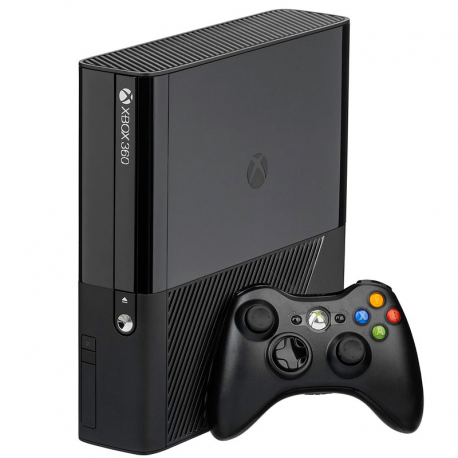
\includegraphics[width=\textwidth]{xbox360.jpg} 
        {\small Xbox 360} 
    \end{column}
\end{columns}

\end{frame}

\begin{frame}
\frametitle{PlayStation 4}
\begin{columns}

\begin{column}{0.6\textwidth}
\textbf {PlayStation 4} – konsola ósmej generacji, stworzona przez Sony Computer Entertainment i wydana 15 listopada 2013 roku w Ameryce Północnej, a następnie w Europie i innych częściach świata.

\vspace{0.5em} 
PS4 była ogromnym krokiem naprzód w stosunku do swojego poprzednika, PlayStation 3, oferując lepszą wydajność, grafikę, a także bogatszą ofertę usług i gier. PS4 została zaprojektowana z myślą o wykorzystaniu technologii PC, co zapewniło jej lepszą wydajność, a także ułatwiło deweloperom tworzenie gier. Dzięki zastosowaniu technologii x86, procesory i układy graficzne w PS4 były bardziej kompatybilne z komputerami osobistymi, co przyczyniło się do rozwoju gier na tej platformie.

\vspace{0.5em}
\textbf {PlayStation VR} (wydane w 2016 roku) stanowiło rozwinięcie technologii VR (virtual reality) dla PS4, pozwalając graczom na zanurzenie się w wirtualnym świecie gier.

\end{column}

\begin{column}{0.35\textwidth}
        \centering
        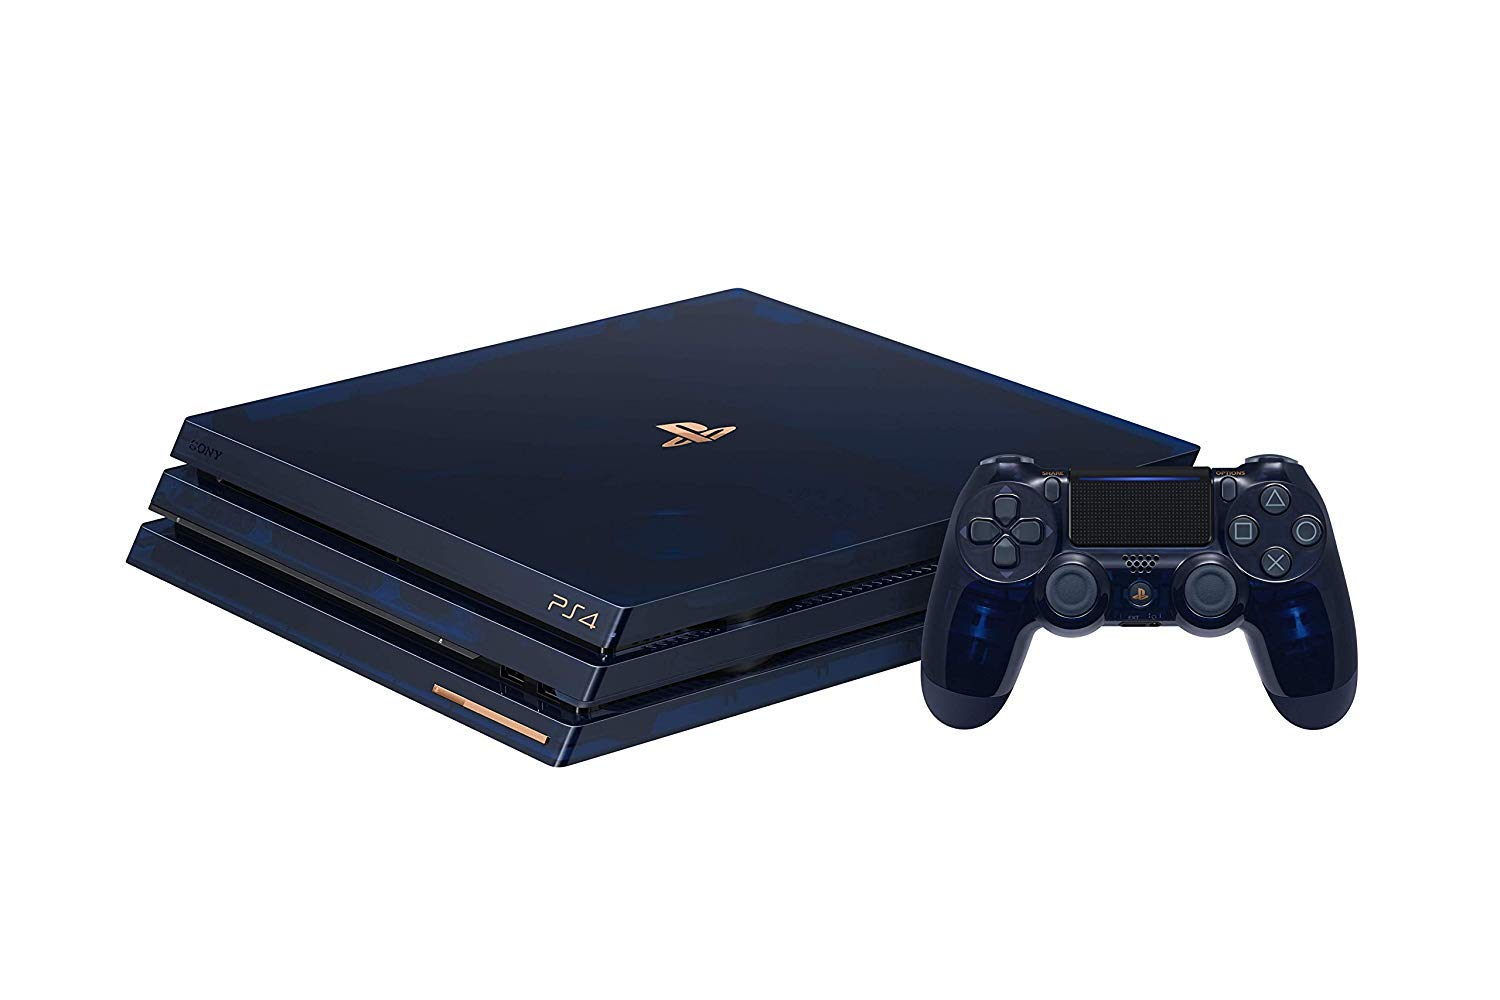
\includegraphics[width=\textwidth]{ps4.jpg} 
        {\small PlayStation 4} 
    \end{column}
\end{columns}

\end{frame}

\begin{frame}
\frametitle{Xbox One}
\begin{columns}

\begin{column}{0.6\textwidth}
\textbf {Xbox One} –  konsola ósmej generacji stworzona przez Microsoft, która została wydana 22 listopada 2013 roku, niemal równocześnie z PlayStation 4. 

\vspace{0.5em} 
Xbox One był następcą Xbox 360 i stanowił część ekosystemu Xbox, który obejmował nie tylko gry, ale także multimedia, usługi online i rozrywkę. Choć początkowo Xbox One zmagał się z kontrowersjami dotyczącymi polityki DRM (Digital Rights Management), z czasem konsola zdobyła dużą popularność, stając się jednym z głównych graczy na rynku gier wideo.

\vspace{0.5em}
\textbf {Xbox Game Pass} (usługa subskrypcyjna) stała się jednym z najważniejszych atutów Xbox One, oferując graczom dostęp do biblioteki gier za stałą miesięczną opłatą. Xbox Play Anywhere to funkcja, która umożliwiała grę na konsoli i PC, bez konieczności zakupu tej samej gry dwa razy.

\end{column}

\begin{column}{0.35\textwidth}
        \centering
        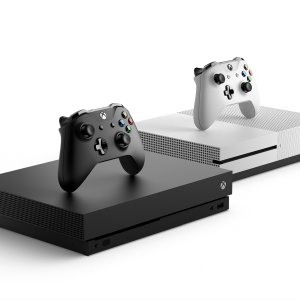
\includegraphics[width=\textwidth]{xone.jpg} 
        {\small Xbox One} 
    \end{column}
\end{columns}

\end{frame}

\begin{frame}
\frametitle{Nintendo Switch}
\begin{columns}

\begin{column}{0.6\textwidth}
\textbf {Nintendo Switch} –  konsola ósmej generacji stworzona przez Nintendo, która zadebiutowała 3 marca 2017 roku. Switch jest wyjątkową konsolą hybrydową, łączącą cechy zarówno konsoli stacjonarnej, jak i przenośnej. To innowacyjne podejście sprawiło, że Switch zdobył ogromną popularność na całym świecie, stając się jednym z najlepiej sprzedających się urządzeń w historii Nintendo, a także na rynku gier ogólnie. 

\vspace{0.5em} 
Dzięki unikalnemu połączeniu elastyczności i wydajności, Switch przyciągnął zarówno graczy casualowych, jak i hardkorowych, oferując szeroką gamę gier, w tym duże tytuły AAA oraz gry niezależne.

\vspace{0.5em}
Konsola Switch jest wyposażona w \textbf {Joy-Con} – dwa odłączane kontrolery, które umożliwiają różne style gry.

\end{column}

\begin{column}{0.35\textwidth}
        \centering
        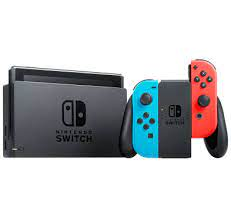
\includegraphics[width=\textwidth]{nswitch.jpg} 
        {\small Nintendo Switch} 
    \end{column}
\end{columns}

\end{frame}

\begin{frame}
\frametitle{Konsole teraźniejszej generacji}

Konsola dziewiątej generacji, czyli PlayStation 5, Xbox Series X oraz Xbox Series S (wszystkie wydane w 2020 roku), reprezentują nową erę gier, oferując znaczną poprawę wydajności, jakości grafiki i technologii, w porównaniu do poprzednich modeli. 
Te urządzenia zostały zaprojektowane z myślą o szybkiej ładowalności, lepszym wrażeniu dźwiękowym i płynnej rozgrywce.
    \begin{figure}[ht]
        \begin{minipage}[b]{0.45\linewidth}
            \centering
            
\includegraphics[width=\textwidth]{ps5.jpg}
        \end{minipage}
        \hspace{0.5cm}
        \begin{minipage}[b]{0.45\linewidth}
            \centering
            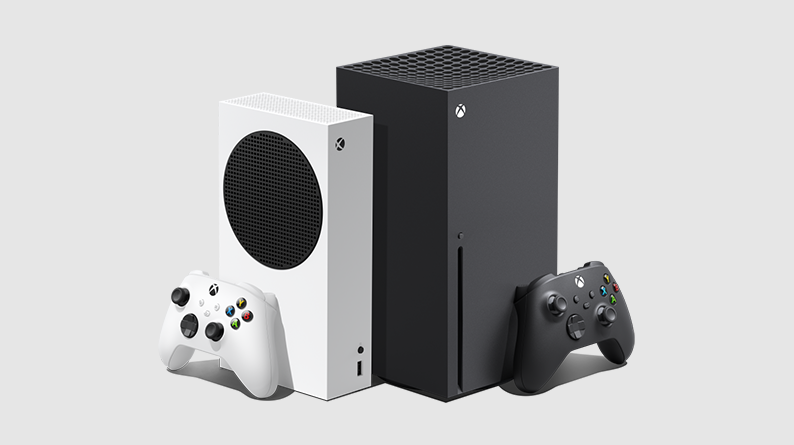
\includegraphics[width=\textwidth]{xseries.png}
        \end{minipage}
    \end{figure}
\end{frame}

\begin{frame}
\frametitle{Podsumowanie}
Historia konsol do gier to fascynująca opowieść o ciągłej ewolucji technologii, która przez dekady zmieniała sposób, w jaki ludzie grają, komunikują się i spędzają czas wolny. Począwszy od pierwszych, prostych konsol takich jak \textbf {Magnavox Odyssey} z lat 70., przez wczesne wersje \textbf{Atari}, które wprowadziły gry wideo do domów na szeroką skalę, aż po przełomowe konsole jak \textbf {PlayStation, Xbox i Nintendo}.
\vspace{0.5em}
Każda generacja konsol wnosiła innowacje w zakresie technologii graficznych, dźwiękowych, a także interakcji z użytkownikami. Począwszy od konsol 8-bitowych, przez 16-bitowe, aż po dzisiejsze urządzenia 4K z ray tracingiem i zaawansowanymi kontrolerami oferującymi nowe sposoby interakcji z grami (np. \textbf {DualSense w PS5}). Technologie takie jak \textbf {dyski SSD}, \textbf {chmurowe usługi gamingowe} czy \textbf {dźwięk przestrzenny} zrewolucjonizowały sposób, w jaki gracze doświadczają wirtualnych światów.
\vspace{0.5em}
Współczesne konsole nie są już tylko urządzeniami do grania – stają się centrum multimedialnym, integrując gry, filmy, muzykę i usługi online. Przyszłość konsol z pewnością będzie związana z dalszym rozwojem wirtualnej rzeczywistości, sztucznej inteligencji oraz coraz głębszym połączeniem z chmurą i usługami streamingowymi.

\end{frame}

\end{document}
